\documentclass{sigchi}

% Use this command to override the default ACM copyright statement (e.g. for preprints). 
% Consult the conference website for the camera-ready copyright statement.


%% EXAMPLE BEGIN -- HOW TO OVERRIDE THE DEFAULT COPYRIGHT STRIP -- (July 22, 2013 - Paul Baumann)
 \toappear{Permission to make digital or hard copies of all or part of this work for personal or classroom use is 	granted without fee provided that copies are not made or distributed for profit or commercial advantage and that copies bear this notice and the full citation on the first page. Copyrights for components of this work owned by others than ACM must be honored. Abstracting with credit is permitted. To copy otherwise, or republish, to post on servers or to redistribute to lists, requires prior specific permission and/or a fee. Request permissions from permissions@acm.org. \\
{\emph{CHI'14}}, April 26--May 1, 2014, Toronto, Canada. \\
 Copyright \copyright~2014 ACM ISBN/14/04...\$15.00. \\
DOI string from ACM form confirmation}
%% EXAMPLE END -- HOW TO OVERRIDE THE DEFAULT COPYRIGHT STRIP -- (July 22, 2013 - Paul Baumann)


% Arabic page numbers for submission. 
% Remove this line to eliminate page numbers for the camera ready copy
% \pagenumbering{arabic}


% Load basic packages
\usepackage{balance}  % to better equalize the last page
\usepackage{graphics} % for EPS, load graphicx instead
\usepackage{times}    % comment if you want LaTeX's default font
\usepackage{url}      % llt: nicely formatted URLs
\usepackage{microtype}
% llt: Define a global style for URLs, rather that the default one
\makeatletter
\def\url@leostyle{%
  \@ifundefined{selectfont}{\def\UrlFont{\sf}}{\def\UrlFont{\small\bf\ttfamily}}}
\makeatother
\urlstyle{leo}


% To make various LaTeX processors do the right thing with page size.
\def\pprw{8.5in}
\def\pprh{11in}
\special{papersize=\pprw,\pprh}
\setlength{\paperwidth}{\pprw}
\setlength{\paperheight}{\pprh}
\setlength{\pdfpagewidth}{\pprw}
\setlength{\pdfpageheight}{\pprh}

% Make sure hyperref comes last of your loaded packages, 
% to give it a fighting chance of not being over-written, 
% since its job is to redefine many LaTeX commands.
\usepackage[pdftex]{hyperref}
\hypersetup{
pdftitle={SIGCHI Conference Proceedings Format},
pdfauthor={LaTeX},
pdfkeywords={SIGCHI, proceedings, archival format},
bookmarksnumbered,
pdfstartview={FitH},
colorlinks,
citecolor=black,
filecolor=black,
linkcolor=black,
urlcolor=black,
breaklinks=true,
}

% create a shortcut to typeset table headings
\newcommand\tabhead[1]{\small\textbf{#1}}


% End of preamble. Here it comes the document.
\begin{document}

\title{Visualisation of Formula One Racing Results}

\numberofauthors{3}
\author{
  \alignauthor Giuseppe Callari\\
    \affaddr{\normalsize Katholieke Universiteit Leuven}\\
    \email{\normalsize  giuseppe.callari@student.kuleuven.be}\\
  \alignauthor Michael Vincken\\
    \affaddr{\normalsize Katholieke Universiteit Leuven}\\
    \email{\normalsize michael.vincken@student.kuleuven.be}\\
  \alignauthor Stefan Pante\\
    \affaddr{\normalsize Katholieke Universiteit Leuven}\\
    \email{\normalsize stefan.pante@student.kuleuven.be}\\
}

\maketitle

\begin{abstract}
This paper describes the design and implementation of a visualisation of Formula One racing results. The user can interact with the visualisation using a draggable timeline. We use coloured bar charts to show a visual representation of the performances of drivers over the years. Moreover, our visualisation gives the user the opportunity to compare two drivers based on their finishing positions per season. Through this paper, we will shortly discuss the problems we have encountered such as the point system for the championship that has been changed several times over the years and that the original data format did not allow for a performant visualisation, which required us to do some heavy preprocessing on the data. At the end of this paper we describe some lessons we have learned in the process of making this visualisation such as the drawing order of SVGs in D3.js and assumptions that were made but were not always correct.

\end{abstract}

\keywords{
Information visualisation; Formula One; Race results; Motor sport; Seasonal wins; Drivers; Constructors; Compare performances
}

\category{H.5.m.}{Information Interfaces and Presentation (e.g. HCI)}{Miscellaneous}





% \begin{figure}
% \begin{center}
% 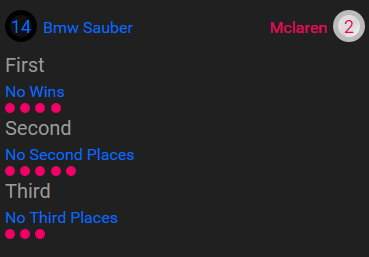
\includegraphics[width=\columnwidth]{images/statistics.png}
% \label{fig:statistics}
% \caption{A screenshot of the statistics corresponding to one year in the timeline}
% \end{center}
% \end{figure}











% \begin{figure}[H]
%   \centering
%   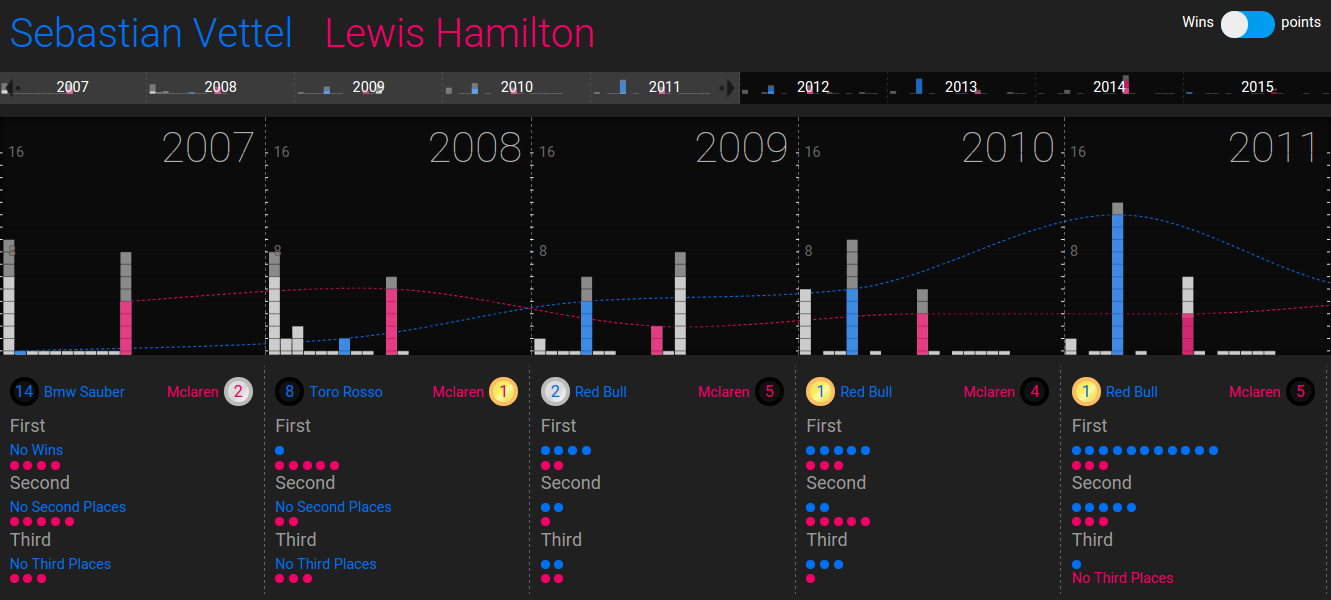
\includegraphics[width=1\columnwidth]{images/top.png}
%   \caption{Alternative layout where the navigator is at the top of the visualisation}
%   \label{fig:top}
% \end{figure}

\section{Introduction}
The FIA Formula One World Championship, better known as Formula One or F1, is one of the most popular motor sports in the world. The F1 season consists of a series of races, also called Grands Prix, held throughout the world. Each season consists of a certain number of races. During a season, a number of teams or constructors (we will use these names interchangeable in this paper) compete with each other. Currently, each team consists of two drivers. After each race, drivers receive points depending on their finishing position. In the current system, the top ten driver-car combinations are awarded points. Based on the racing result of the drivers at the end of the season, the team with the highest cumulative score wins the constructors title and the driver with the highest individual score wins the World Championship title.
 
There already exist visualisations for consulting the statistics of Formula One racing results\cite{lapchart}\cite{spenke2000infozoom}. Most of these visualisations give the user an overview of results per season. The specific focus of our visualisation is that we want to make it easy to compare driver results over several years.
 
The goal of this visualisation is to present an overview of seasonal race results for specific drivers throughout their active years, while keeping an overview of the opponents. This visualisation is interesting for motor sport fanatics or those who want to know more about a driver’s performance. A minor understanding of Formula One is required.
 
In this paper, we first give some background information about Formula One racing statistics. Next, we describe the data set we used for our visualisation. Then we discuss the technology used for the visualisation. Afterwards, we describe the different parts of our visualisation. Finally, we discuss some future and related work. 

\section{Formula One Racing Statistics}
As stated previously, a Formula One racing team consists of several drivers. In general, two drivers are the main drivers of the team. The other drivers are test drivers or can take the place of one of the two main drivers in case one is not able to participate in a race (due to medical conditions or a disqualification). Note that these regulations are the current ones. In the pre-modern Formula One era (pre 1970), more than two drivers per team could participate in a race\cite{wiki}. We noticed this in the final stages of development. Therefore, we state that this visualisation is not a tool to compare constructors, unless for the most recent seasons. We only show the the two best drivers of each team.  Each driver can earn points in a race when finishing in the top 10. In the current point system, the winner gets 25 points, the second 18 points, third 15 and so on. It is important to note that the scoring system has been changed several times over the years\cite{wikipoints}. This complicates comparison over over the years. This is why we choose to discard the original points that each driver has earned and used the current point system for all drivers instead.

\section{Data Set}
For our visualisation, we made use of the Ergast API\cite{ergast}. The Ergast API provides data for the Formula One and Formula E series from the beginning of the world championships in 1950 and 2015 respectively. Data can be requested in different formats: XML, JSON and JSONP. We opted to use JSON because it can be directly used in javascript without the need of parsing. 

A problem we encountered was that the Ergast API only provides data about the lap times starting from 2008. We did not find any other source which provided this kind of information. To overcome this problem we decided to focus on driver performance through the years. This data was readily available because the API supports requests for statistics per race or per season for both the drivers and the teams. Despite not containing all the data we originally wanted, the Ergast API was the most detailed source of Formula One statistics we could find without resorting to building  a web scraper. 

The API was used to build our own static dataset. A direct connection between the visualisation and the API was not possible due to the multitude of requests necessary to get all required data. This would result in unacceptable slow behaviour. More about how we used the API to build our own dataset is detailed in the Section \nameref{gathering}. 

\subsection{Data Analysis} 

\begin{figure}[ht]
\centering
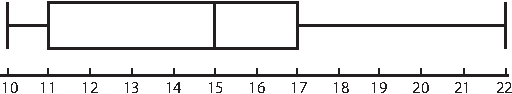
\includegraphics[width=0.8\columnwidth]{images/constructorsboxplot.pdf}
\caption{Box plot of the number of constructors per year}
\label{fig:constructorsboxplot}
\end{figure}

\begin{figure}[ht]
\centering
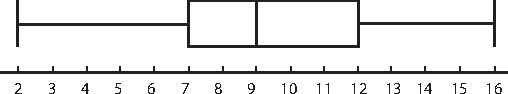
\includegraphics[width=0.8\columnwidth]{images/winsboxplot.pdf}
\caption{Box plot of the career lengths of drivers with wins in their career}
\label{fig:winsboxplot}
\end{figure}

\begin{figure}[ht]
\centering
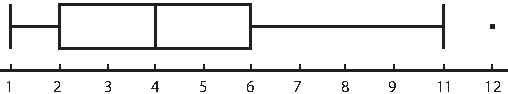
\includegraphics[width=0.8\columnwidth]{images/pointsboxplot.pdf}
\caption{Box plot of the career length of drivers with points in their career}
\label{fig:pointsboxplot}
\end{figure}
In order to get 
more insight in our dataset, we performed some data analysis. The number of drivers who didn’t earn a single win/point in their career was calculated. This number is large (728 drivers never won, 504 never scored any points). This is not a problem for the visualisation because we are only interested in the careers of drivers who performed well. Consequently the drivers with no wins/points are not of interest and are not visible in our visualisation. To be able to further refine the data analysis, we made box plots for the number of teams per season (Fig. \ref{fig:constructorsboxplot}), the length of the careers of drivers with points/wins(Fig. \ref{fig:pointsboxplot} and \ref{fig:winsboxplot}). This showed us that the maximum amount of teams we had to visualise per season was 22, which is a reasonable amount for the amount of space allowed per season in the timeline. Furthermore, the analysis of the average career length of drivers with wins/ points shows us that the average career length of a driver with points in his career is 5.01 and 4.30 when outliers are removed from the data (normalized to current point system). The average career length of a driver with wins is higher at 9.30. The average career length of drivers with wins is too high too be displayed on one screen, since it would make the timeline too dense (see Figure \ref{fig:numYears}). we choose to display five seasons on one screen because it matches the career length of drivers with points and evenly distributes the average career length of drivers with wins across two screens.

\begin{figure}[ht]
\centering
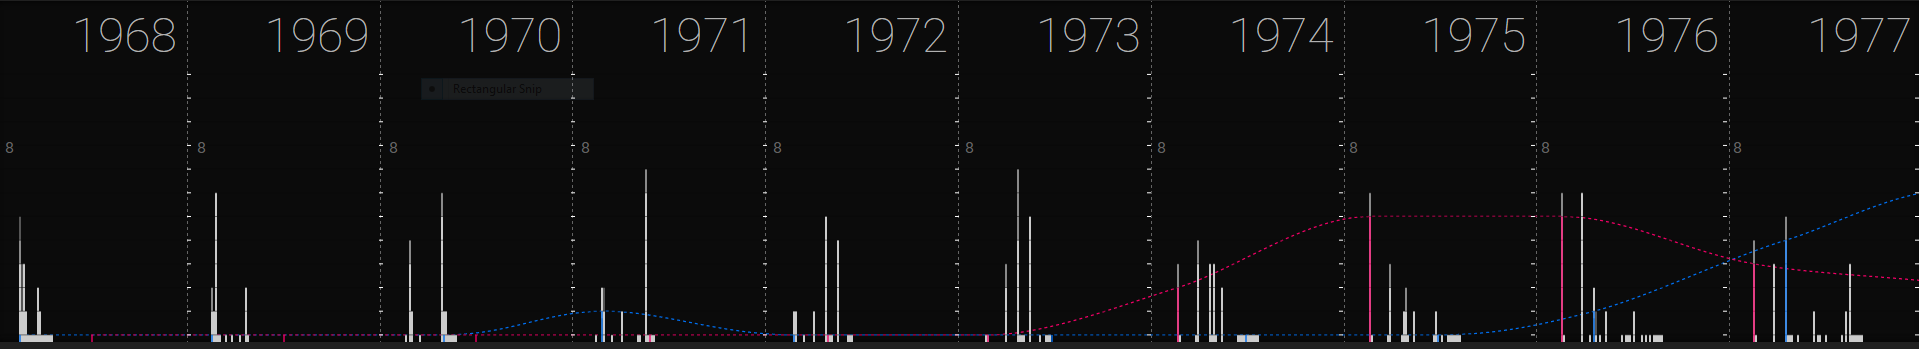
\includegraphics[width=1\columnwidth]{images/dense.png}
\label{fig:numYears}
\caption{Figure illustrating how the timeline looks when ten years are visualised at the same time}
\end{figure}

\section{Our Visualisation}
\begin{figure*}[tp]
  \centering
  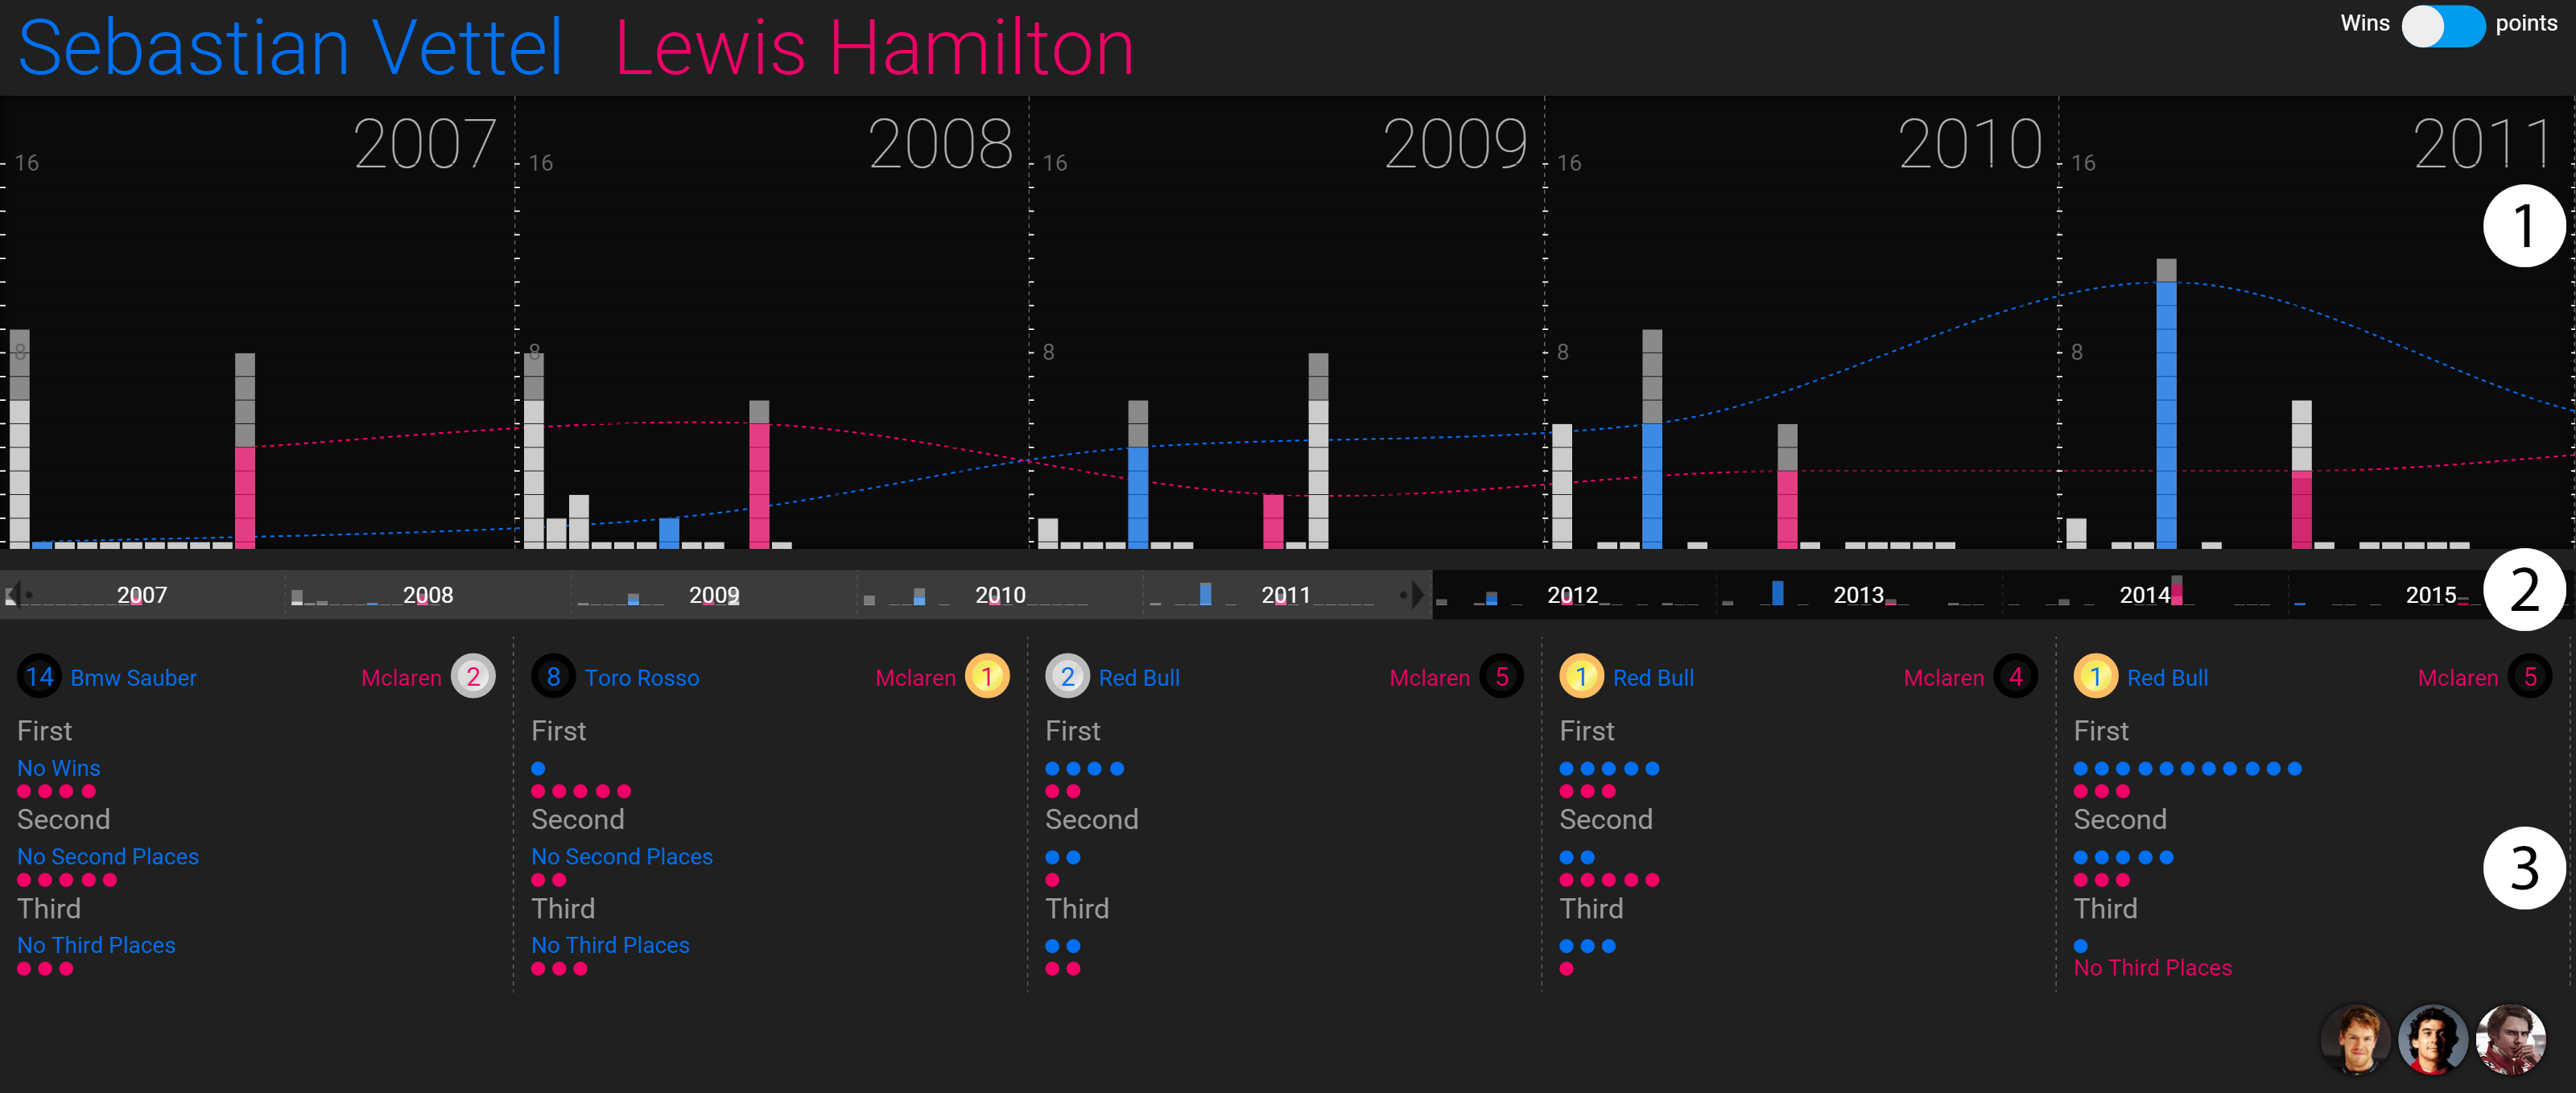
\includegraphics[width=1\textwidth]{images/overview.png}
  \caption{Overview of our visualisation showing (1) the timeline, (2) the navigator and (3) the statistics}
  \label{fig:overview}
\end{figure*}

\begin{figure}[ht]
  \centering
  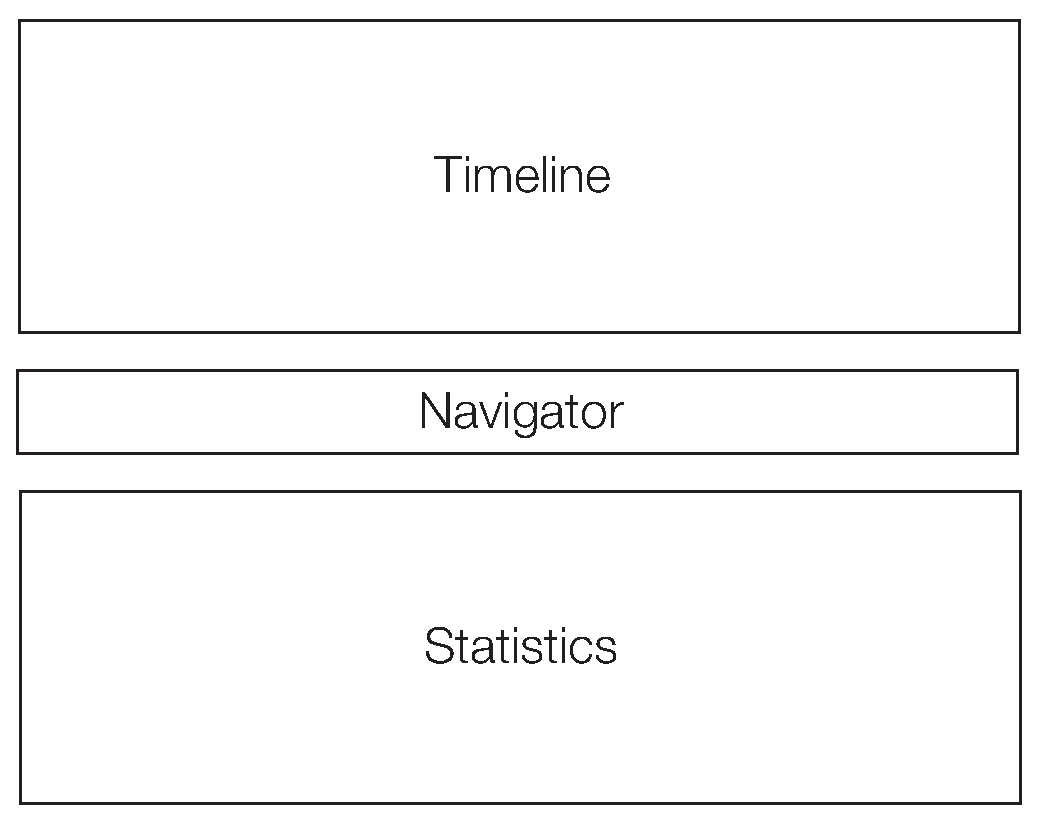
\includegraphics[width=0.75\columnwidth]{images/layout.pdf}
  \caption{Overview of our visualisation showing (1) the timeline, (2) the navigator and (3) the statistics}
  \label{fig:layout}
\end{figure}
Our visualisation consists of three parts as shown in Figure \ref{fig:overview} and \ref{fig:layout}: the timeline is the main part of our visualisation where we provide a five year view of seasonal wins or points for the different drivers grouped by constructor. The second part is the navigator. The draggable bar of the navigator is used by the user to change the view to a period of interest. The third part, located under the timeline, focuses on two specific drivers to enable a comparison of their performance based on podium finishes (first, second or third places). This part, called the statistics section, also shows the final ranking of a selected driver in a season . 

\subsection{Timeline}
\label{timeline}



The timeline contains the active years of the selected driver. For each year, we plot the number of wins or points using stacked bar charts. Each stacked bar represents a constructor who competed for the title in that specific year. Figure \ref{fig:stacked} illustrates that a bar is divided in two colours, namely dark and light grey. The light gray bar, the bottom part, represents the number of wins or points – depending on the selected metric –  of the driver who performed the best for that team. More specifically, this bar represents the driver who has earned the most points or wins during the season. The dark grey bar, the upper part of the bar, represents the number of wins or points of the best other driver from the same team. These two bars are stacked on top of each other. We believe that designing the non selected drivers in this way results in a more consistent visualisation. Making the stack order random would be a confusing factor and could interfere with our goal of visualising information in a clear way. By using stacked bar charts, we visualise the individual wins or points of the drivers and which drivers were together in a team. The performances based on the criterium of wins points are represented by the height of the bars corresponding to the drivers. Details are provided by hovering on the bars using tooltips.

\begin{figure}[ht]
\centering
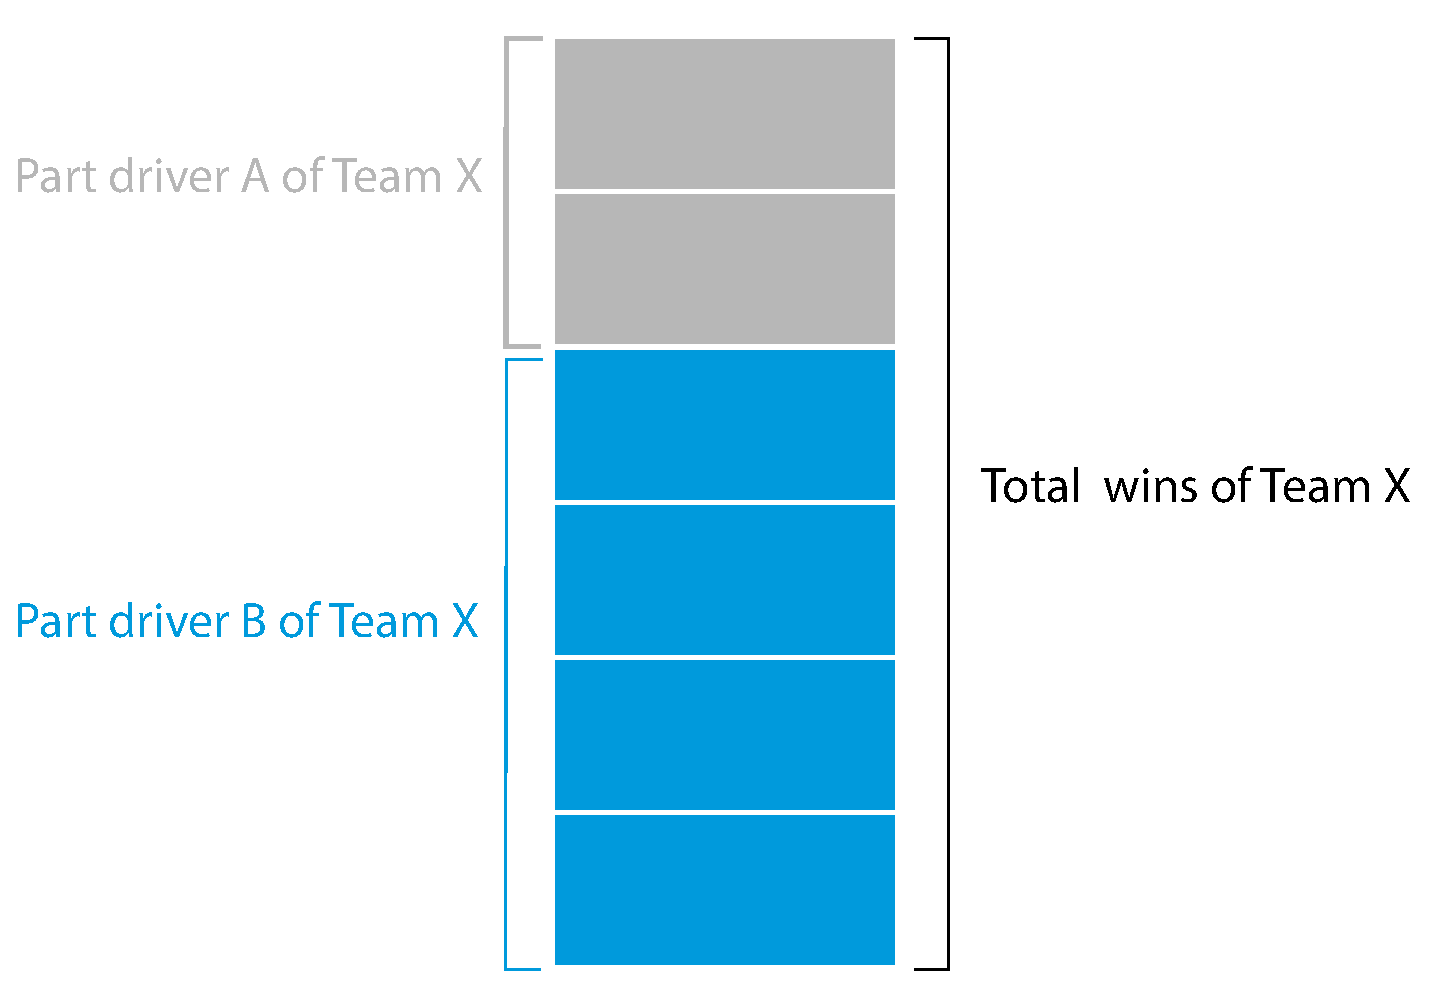
\includegraphics[width=0.75\columnwidth]{images/stackedbar.pdf}
\caption{Illustration of a stacked bar in our visualisation}
\label{fig:stacked}
\end{figure}
 
When the user hovers over a part of a bar in the timeline, a tooltip pops up and displays the name of the corresponding driver, as well as his number of wins or points.  By clicking on that part of the bar, the data of the corresponding driver is loaded and the visualisation in the lower part is updated. The visualisation in the lower part is the statistics view discussed in the Section \nameref{statistics}. Before the data of a new selected driver is loaded, the user must choose which already selected driver must be substituted by the new one. This is done by a small dialog window.

Bars corresponding to the selected drivers are visualised in a color different than the not selected ones in order to put them in focus. The same colors are used for the corresponding name (upper left in Figure \ref{fig:overview}), the trend lines (discussed in the Section \nameref{trend lines}) and the statistics (discussed in the Section \nameref{statistics}).

The bars of selected drivers must start at the same position (the bottom of the timeline) to compare their heights. Starting at the bottom has the consequence that the performance can be read on the provided vertical axis.

Our timeline is in fact a two-dimensional graphic with one dimension used to represent time and the second to represent a magnitude associated to the events represented. In our visualisation, the events are the performances of drivers. According to J.Y Blaise et al.[9] , this representation of time is easy to read; it usefully enhances comparisons, cross examination of indications, and allow for magnitude assessment.  Furthermore, they call this kind of timeline a time chart. 


\paragraph{Alternatives}

Cleveland et al.\cite{cleveland1984graphical} prefer to replace stacked bar charts by grouped dot charts. This makes comparing drivers of a same team easier: length judgments are replaced by position judgments. However, we already sort drivers belonging to the same team: the best driver is placed at the bottom, if the team does not contain a selected driver. This visualisation technique shows the user which driver was the best driver in a team. If a selected driver is present, he is placed at the bottom instead. Notice that a best non-selected driver is always represented by a light gray bar, even if his team member is selected. Hovering is used to reveal the wins or points of a driver. Furthermore, if we replaced the stacked bar charts by grouped dot charts, more space would be  needed on the axis that represents time.

\subsubsection{Trend lines}
\label{trend lines}
The trend lines for the selected drivers are added to assist the user when comparing the selected drivers. For each selected driver, a trend line is drawn adjacent to the corresponding bars. In each year, the bar of a selected driver is surrounded by bars representing his competitors. This trend line is used to connect all the bars for a selected driver and thus to visualise the career of a selected career more explicitly. We believe that adding this trend line improves the clarity when comparing careers and when analysing one particular career, since the bars of one driver are not placed near each other. Crossing trend lines make clear that one driver surpasses the other. Furthermore, an increase or decrease in points or wins is indicated by a positive or negative slope of the trend line. 


\subsection{Navigator}

A draggable bar is added beneath the timeline for easier navigation (see Figure \ref{fig:overview} ), called the navigator. Inside the navigator, a miniature version of the bar charts for each year is displayed to give a quick overview. A draggable slider is placed on top to navigate through the years.
This miniature version shows the timeline as a whole, from the beginning to the end without sideways scrolling. This provides an overview for the user. The miniature version does not aim to provide all the information to the user, but it rather is an incentive for the user to explore certain periods. 

It could for example trigger the user to drag the navigator to the start of some driver’s career when exploring the end of it. The start could have same peaks which the user did not remark on the visible section of years of the main timeline. Visualizing the distribution of the data and showing individual data values in the navigator is proposed by Stephen G. Eick\cite{eick1994data}: “Linking sliders to the data they control suggests many natural and obvious extensions.”



\paragraph{Alternatives}
\begin{figure*}[tp]
\centering
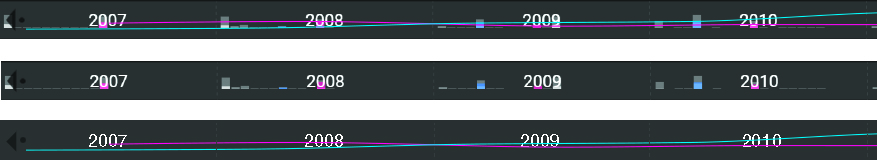
\includegraphics[width=1\textwidth]{images/navigators.jpg}
\caption{Alternatives for the navigator which show the trend line with barcharts, only barcharts and only trend line}
\label{fig:navigator}
\end{figure*}

We considered two alternative representations for the navigator in which the bar charts are replaced or accompanied by a miniature version of the trend line for the two selected drivers. Mock-ups of these alternatives are shown in Figure \ref{fig:navigator}. A drawback of the usage of the trend line is that the difference between the performance of the drivers over the years becomes less obvious because of the small scale of the navigator. Another drawback is apparent if we only use the trend line: the information about the drivers other than the selected is lost.
The alternative with both the trend line and bar charts shows more data, but obstructs the view for the user and exploring the timeline becomes more cumbersome.


\subsection{Statistics}

\label{statistics}
Below the timeline and the navigator, another section is visualised in parallel. This line is divided in year blocks similar to the timeline. In every block, more information about the selected  drivers is shown. These blocks are reserved for analysis of the selected drivers only. Three metrics are compared: number of first places, number of second places and number of third places. These correspond to rankings for which a driver is allowed on the podium during the podium ceremony. During this ceremony, the best three drivers are celebrated after each race. Podium finishes are considered an important statistic used in sports to analyse an athlete's career (or driver's career in motorsport). Achieving a podium finish puts the driver in the spotlights by honoring its achievement publicly. During the olympics, medals and thus podium places are an important metric as well. Countries are usually ranked by the number of medals achieved by their athletes \cite{olympic}. MotoGP, the premier class of GP motorcycle racing\cite{motogp}, provides a search functionality on its official website in order to let user explore their database of races, drivers and results. ``Podium with riders of the same nation'' is a search space users can explore.

For each podium finish (first, second and third), the number obtained during that season is visualised using circles. The color of a circle corresponds to the driver. Each place has two horizontal rows of circles, in which each driver corresponds to a row. Furthermore the names of the constructors of the drivers are shown as well. The position and color of the constructor corresponds with the selected driver. The position in the block corresponds to the position of the name of the driver shown in the left upside corner of the visualisation. A medal indicating the final ranking is placed next to the team name for the corresponding year. A first place and thus championship win is decorated with a gold medal, a second place is decorated with a silver medal, a third place is decorated with a bronze medal and a place lower than three is decorated with a dark blue medal. In each medal, the number corresponding with the finishing position in the championship is shown.



\subsection{Points versus wins} 

In the initial design of our visualisation number of wins were used to determine the height of the bars of the different drivers. We opted to use the number of wins of a driver in order to compare drivers because this metric that has not been changed over the years. In contrast with  the number of wins, the score system has changed several times over the years\cite{wikipoints}. Therefore, this metric is not ideal to compare drivers in the main timeline which competed in different periods. To overcome this problem we normalised the score systems to the system used in the year 2014. This way we give the user the opportunity to compare two drivers based on their points. A driver who has won the most races does not always has the most points and therefore did not win the championship of that year. The user can easily switch between the points and wins of the selected drivers to review their season by using the toggle shown in the upper right of Figure \ref{fig:overview}. We believe that the statistics beneath the timeline provide the context to interpret results of drivers and that they can be an incentive to change the view. Let us consider drivers who achieved none or very few (one or two) wins. These drivers however could have achieved many podium places during a year. Second and third places have always be rewarded by points. Changing the view will reveal the gathered points. 


\subsection{Layout} 
\label{layout}
As shown in Figure \ref{fig:overview}, our visualisation consists of three parts: The timeline, the navigator and the statistics. The navigator is positioned between the statistics and the timeline. Notice that the statistics are positioned beneath the timeline and that each block in the statistics corresponds to a year in the timeline. 
The navigator has the role to summarize and give a global overview of the careers of the selected drivers. It does not show a detailed view, but can be used to pinpoint interesting events in a driver’s career by displaying significant raises and drops in the careers of the selected drivers. This gives the user the possibility to remark these significant changes, even if the current visible section of the timeline does not cover the corresponding years.

The reason we put the navigator between the statistics and the timeline, has no hard foundation based on design patterns proposed and accepted by the information visualisation community. The design decision is based on the conceptual difference between the statistics and the timeline. The navigator is used as a separation between these two parts.


\paragraph{Alternatives} 

\begin{figure}[ht]
  \centering
  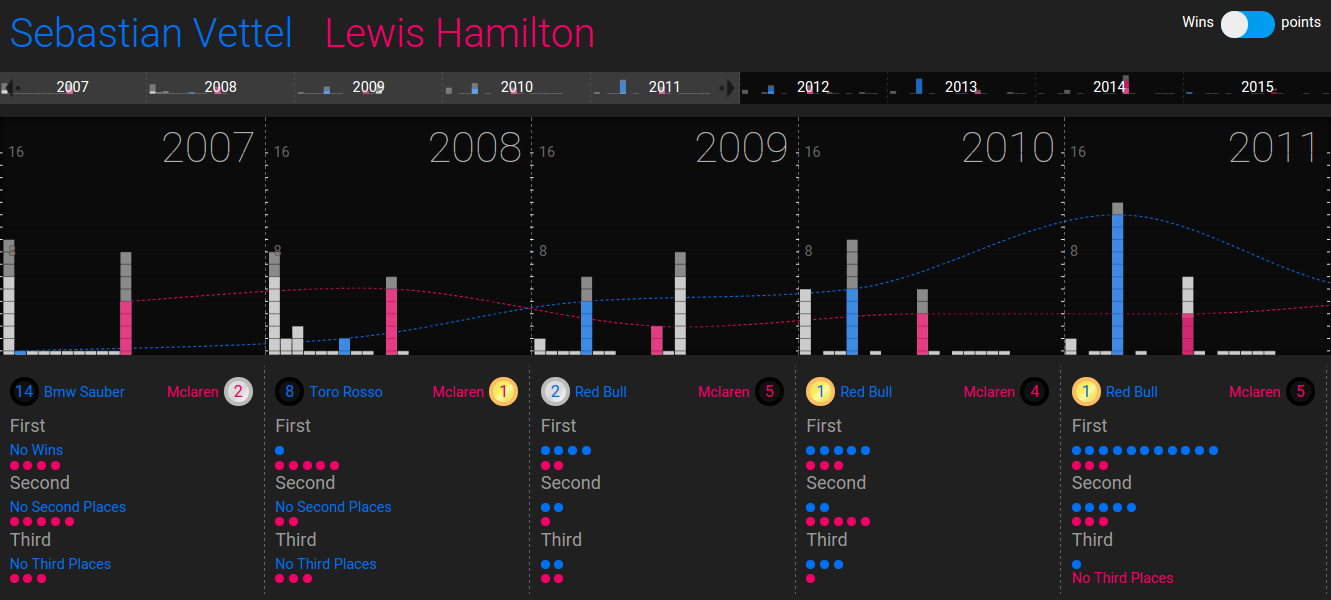
\includegraphics[width=1\columnwidth]{images/top.png}
  \caption{Alternative layout where the navigator is at the top of the visualisation}
  \label{fig:top}
\end{figure}
Some alternatives were considered during development for the layout. See Figure \ref{fig:top}. This alternative shows the navigator at the top. This representation shows a more hierarchical, top down order in which the navigator presents a global overview. Below the navigator, the timeline shows a more detailed view on the data. At the bottom, the statistics are shown. They show even more detail and provide context to the timeline, the backbone of our visualisation. 

Another alternative is to put the navigator at the bottom of the visualisation, which would cause the detailed view of the timeline and statistics to presented at the top and the global overview to be positioned at the bottom. The first alternative seems to be the better if we adhere to the principal of overview first\cite{shneiderman1996eyes}.

The Budgets Forecasts discussed by Edward Segel et al.\cite{segel2010narrative} presents a slider, placed at the bottom, to navigate through the years.  This navigation does not correspond to ours: when sliding from past to present, the user sees more of the line graph. If the slider is put on the present, the whole graph is shown. Hovering over the graph reveals details-on-demand, a design principle we also respected, as discussed in the Section \nameref{timeline}

Furthermore, sliding our navigator zooms in to the selected period of time. Thus, the whole visualisation respects the overview first, zoom and filter, then details-on-demand design principle\cite{shneiderman1996eyes}.



\section{Implementation} 

The implementation of the visualisation consists of four parts: data gathering, the navigator, the timeline and the statistics.


\subsection{Data gathering} 

\label{gathering}
We used the Ergast F1 API to gather our data. We originally planned to connect directly to the API to retrieve the necessary data. It quickly became apparent that a direct connection was not suitable because of the structure of the API. Because our visualisation aggregates a lot of data, too many requests would be required, which would have resulted in very poor performance, numerous time-outs and overall, a worsened user experience. After downloading a database dump, the reasons for the bad performance were immediately clear. The relational database was heavily normalised, requiring multiple joins for each API call we made. We opted to transform the data to a JSON-object representation, which is downloaded in its entirety every time a user accesses the visualisation. Uncompressed, the JSON file is roughly 400 KB in size, if the server has gzip compression enabled, the file size is further reduced to 50 KB We chose this approach instead of using a backend NoSQL database because we strongly believe such a database would not provide additional benefits to our users and we wanted to adhere to the KISS principle.

We developed a Node.js and Python script to collect our data. These scripts automate the collection and transformation of our data. The drawback is that the scripts should be run each week to keep the data up-to-date, a process which also could be easily automated on a server.



\subsection{Navigator} 

The navigator is implemented without using a specialised library. We used JavaScript in combination with jQuery, in order to manipulate the CSS and for the implementation of the navigator. The miniature timeline, which shows all the bar charts (selected and not selected drivers of all the years) does not have all the functionality the main timeline provides: the stacked bars are not clickable, nor hoverable and there are no trend lines for the selected drivers visualising the up and downs of their careers. The aforementioned functionalities would not only be redundant for the mini timeline, but would also interfere with the user’s navigation, e.g. clicking on a year in the navigator redirects the user to the corresponding year  in the timeline.

Therefore, the code is not the same as the code for the main timeline. Making the code reusable, and thus avoiding code duplication, resulted in conflicts between svg-elements which were easily fixed by just duplicating the d3 code for the timeline. After duplication, refactoring followed in order to scale and place the miniature timeline under the navigator and in order to remove redundant functionality. 



\subsection{Timeline} 

The timeline which holds all the bar charts is the backbone of our visualisation and its functionality is completely implemented using the d3.js framework. First, the data concerning the not selected drivers is visualised: these are represented by the grey stacked bar charts. Subsequently, the selected drivers are plotted, in a different color. 

The decision to draw the bar corresponding to the best driver (depending on the chosen metric) at the bottom of a stacked bar has a consequence for our gathered data. The data concerning the selected drivers and all drivers who competed in the same years is processed and manipulated before it is visualised: the drivers of a team are sorted by the number of wins or points for each year. This is not done in the data gathering step, but processing the data after gathering them takes care of this sorting step.

After this step, the selected drivers are visualised on the timeline. The bars representing the selected drivers have a different color than the non-selected ones and are always shown as the bottom bar in a team, even if a non selected team-mate had most wins or points in the team. This is discussed in the Section \nameref{timeline}.

Finally, the trend lines are drawn, which complement the bars of the selected drivers. The lines hit the top of the bars of the selected corresponding drivers.

To show which bar corresponds to which driver, we implemented tooltips using the library d3-tips\cite{records} written by Justin Palmer. When hovering over a bar, the bar lights up and the name of the corresponding driver is shown together with the amount of wins or points and the team to which it belongs.



\subsection{Statistics} 

The process of creating and displaying the statistics underneath the timeline is handled by a template engine.Traditionally, the programmer would create new elements by building a string representation of the HTML required and appending it to the DOM. The template engine automates this process, which allows the developer to separate HTML from javascript. 

There are multiple template engines available. Two well known examples are Handlebars\footnote{http://handlebarsjs.com/}  and EJS\footnote{http://www.embeddedjs.com/}. We opted for the EJS template engine because it allows for complex javascript statements inside a template, while Handlebars does not allow complex statements by default. 

Information about the two drivers' championship position, wins, second and third places for each year are given as input in the template engine as a JSON object, together with an URL pointing to the template. The output of the template engine is a representation of the statistic in string format that can easily be appended to the DOM.



\section{Lessons Learned}

When implementing the visualisation, we have dealt with some bottlenecks by not coding as generic as possible. For example, the overview shown in the navigator is implemented by reusing code of the timeline, keeping in mind that not all functionality (hovering, tooltips, selecting a new driver…) of the timeline must be supported by the navigator. During development, changes were made to our timeline. These changes were not forwarded to the navigator, which needed to be refactored. This was time consuming.
Another problem we faced was the drawing order of our SVGs. Our visualisation is composed out of different SVGs e.g. the bar charts, the trend line, etc. If our SVGs are drawn in the wrong order, some bars, located under the trend line were not clickable anymore.



\section{Future Work} 
\begin{figure}[ht]
  \centering
  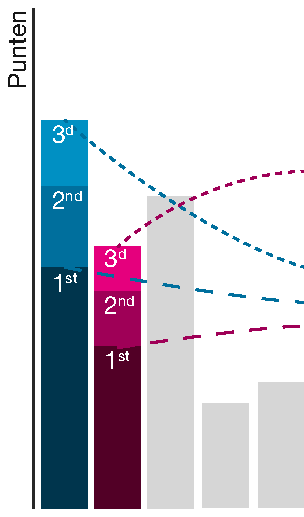
\includegraphics[width=0.5\columnwidth]{images/alternative.pdf}
  \caption{Alternative where every driver has his own bar to show their points,
  the different stacks represent the finishing positions contributions to the points}
  \label{fig:alternative}
\end{figure}

\begin{figure}[ht]
  \centering
  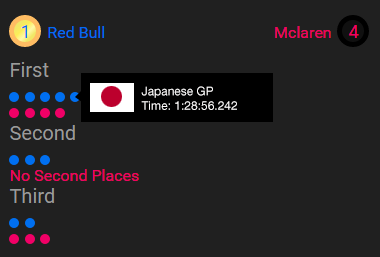
\includegraphics[width=1\columnwidth]{images/hovering.png}
  \caption{Hovering over a win would show more information}
  \label{fig:hover}
\end{figure}

More detail about the wins, second and third places in the statistics can be shown. We could add the grand prix for each of the these places by creating a hover function (see Figure \ref{fig:hover}).
As stated in the beginning of this paper, we found out that there were cases where more than two drivers competed for the same constructor. Our visualisation does not work properly in this situation. Therefore we made a mock-up (see Figure \ref{fig:alternative}) suggesting an alternative way of visualising racing results. Here, each bar represents one driver. The bar is divided in three parts representing the share of his finishing positions contributing to his total points. This way we overcome the problem of grouping drivers per team and at the same time give more information about the performances of the individual driver. A drawback of this way of visualising is that a user does not have an overview of team performances since the drivers are visualised individually.



\section{Related Work}

For related work, we focus on visualisations that represent an overview of results from sports. In the first visualisation, Marcelo Duhalde visualised the FIFA Ranking For The Gulf National Teams\cite{fifaranking}. Duhalde uses a hemisphere to represent a timeline with all the years in which a championship was organised. The y-axis represents the position of the soccer teams at the end of a season. This is an interesting way for visualising scores throughout the years. Marcelo Duhalde used data from 1993 until 2014 to visualise 20 years of soccer championships. Our data ranges from 1960 until 2015. As a result of our data analysis, we opted that it’s clearer to use a draggable timeline instead of a hemisphere. The user can interact with our timeline by using the navigator.  

Another interesting visualisation is the Formula 1 Lap Charts by David Ortiz\cite{lapchart}, which also relies on the Ergast web service for the dataset. This chart visualises the performance of the Formula 1 pilots in the first Grand Prix of the year. The x-axis includes a vertical line for each lap of a specific race. When we expand this visualisation for one full season instead of one race we can clearly see the fluctuations in the scores of the pilots. By following one line you can see the switches in position for that driver. These fluctuations are very interesting to get an overall view of the performances of certain drivers. We used this kind of visualisation as well for our trend line .

As discussed in the the Section \nameref{layout}, The Budgets Forecasts discussed by Edward Segel et al. \cite{segel2010narrative} makes use of a slider to navigate from past to present. But instead of focussing on a period of time, the trend line is more revealed as the user navigates to the present.

\begin{figure}[ht]
  \centering
  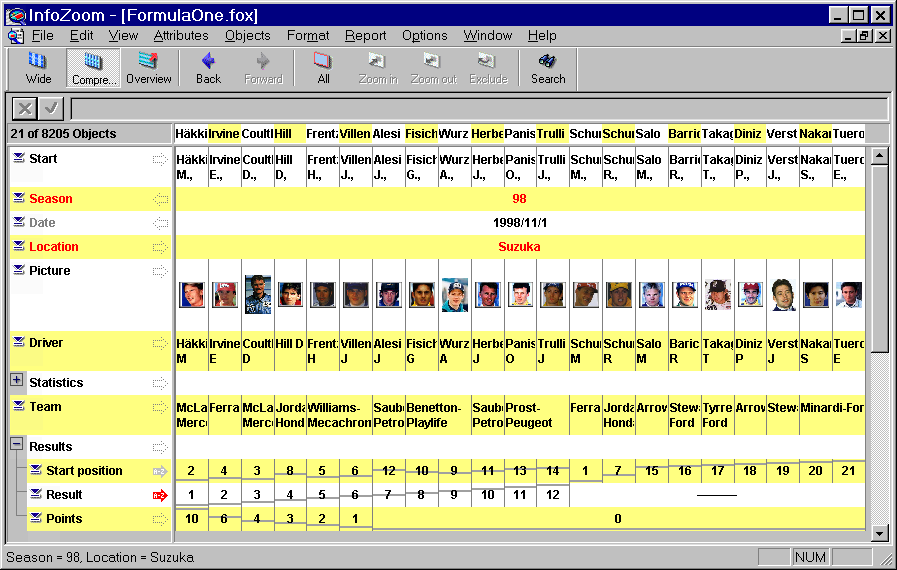
\includegraphics[width=1\columnwidth]{images/infozoom.png}
  \caption{The visualisation tool InfoZoom}
  \label{fig:infozoom}
\end{figure}


Spenke et al.\cite{spenke2000infozoom} visualised Formula One racing results of the last 20 years using a visualisation tool called InfoZoom. This tool is not dedicated to visuations of Formula One data, but is generic and can be used to visualise any relational database. This tool visualises more data than our visualisation e.g. our visualisation does not visualise starting positions. However, it generally uses numbers and horizontal lines to show data. We use stacked bar charts in which bars of selected drivers are colored, trend lines and circles in the statistics. Details-on-demand are achieved by using tooltips in our visualisation. In Figure \ref{fig:infozoom}, a Compressed Table Mode view is shown.


Burch et al.\cite{burch2008timeline} present Timeline Trees to visualise transactions between elements. As an example, they visualised a football game between Germany and the Netherlands during the 1990 World Cup. This technique could be applicable on data of a single race or a single championship, in which position switches are visualised. For yearly data, which we use, using this technique seems more difficult since each season does cover the same drivers. 

A visualisation by General Electric\cite{records} presents an overview of all records for summer Olympic events, in which every circle corresponds to a record. Details about a record are shown when hovering over it. We use the stacked circle approach to visualise the number of first, second and third places. Showing details about a podium finish by hovering over it, is future work.  

Blaise et al. \cite{blaise2008experimenting} describe the evolution of their approach the visualise the city of Krak\'ow and the changes it endured over time. In a first approach, navigating using their timeline showed a view of Krak\'ow corresponding to the selected year. This design did not make it possible to compare two years since only one was shown. 



\section{Conclusion} 

In this paper we described the process for developing our visualisation about Formula One racing results, which consists of three parts. The user can drag the navigator in order to compare two selected drivers. In our visualisation we used bar charts and line charts to visualise the racing results. Each team is visualised by a stacked bar chart, the drivers for that team, in the timeline. This is the backbone of our visualisation. The bars either show the number of wins or gathered points, depending on the chosen metric to compare two drivers. This metric can be switched by the user using the toggle. Extra statistics are used to provide context to the visualised data in the timeline. We believe that our visualisation is a good way of visualising racing result over time where a user can easily compare drivers (and constructors) based on their performances.



\bibliographystyle{SIGCHI-Reference-Format}
\bibliography{bibliography}


\end{document}
